\documentclass[11pt, conference]{IEEEtran}
\usepackage{xeCJK}
\usepackage{amsmath}
% 用来断词,当出现花括号中的单词时,若遇到换行需要断词的话就只能从-处断。
\hyphenation{op-tical net-works semi-conduc-tor}

\begin{document}
    \title{Report of Chapter 2: Temporal Logic}
    \author{\IEEEauthorblockN{林奇峰, Qifeng Lin}\IEEEauthorblockA{Student ID:17214656}}
    \date{\today}
    \maketitle

    \section{Review}
    In this paper, it mainly demonstrates the grammar and advantages of $\text{CTL}^*$.

    $\text{CTL}^*$ is the abbreviation of {\itshape "Computation Tree Logic"} and a kind of temporal logic which is used to describe properties concerned with the executions of a system.
    Firstly, the grammar of $\text{CTL}^*$ is introduced, which can be divided into two parts——one is expressed along a execution (or path) and another one along the set of executions. The first part involved atomic propositions, boolean combinators, temporal combinators, and $\cup$ combinator while the second one consists of path quantifiers. All these will be explained as following:
    \begin{itemize}
      \item Atomic propositions are used to label corresponding states, behaving similarly in automaton $\mathcal{A}$ of chapter 1. They have well-defined truth, that is, they are either true or false and a proposition is true only and only if $P \in l(q)$.
      \item Boolean combinators are comprised of constants \textbf{true} and \textbf{false},, $\neg$, $\wedge$, $\vee$, which are very commonly used in first-order logic.
      \item Temporal combinators are used to describe a sequence of states in an execution and the simplest combinators are $\text{\textbf{X}}$, $\text{\textbf{F}}$ and $\text{\textbf{G}}$, where $\text{\textbf{X}}P$ means that along the execution, the next state should satisfy $P$, and $\text{\textbf{F}}P$ states that along the execution in the future, there will be a state satisfying $P$ and $\text{\textbf{G}}$ means that all states along the execution should satisfy $P$. By the way, $\text{\textbf{G}}\phi$ is equivalent to $\neg\text{\textbf{F}}\neg P$.
      \item $\text{\textbf{U}}$ combinator if often expressed in the form of $\phi \text{\textbf{U}} \psi$ and it means that $\phi$ is verified until $\psi$ is verified, that is, only after $\psi$ happened, $\phi$ can be verified. And there exists "weak until" ($\phi \text{\textbf{W}}\psi$) which does not require the occurrence of $\psi$ and under the condition, $\phi$ remains true.
      \item Path quantifiers includes $\text{\textbf{A}}$ and $\text{\textbf{E}}$. The former in the form of $\text{\textbf{A}}\phi$ states that all executions from the current state should satisfy $\phi$ and the latter in the form of $\text{\textbf{E}}\phi$ means that from the current state, there exists an execution which can satisfy $\phi$. $\text{\textbf{A}}$ and $\text{\textbf{G}}$ both have the meaning of "all" but $\text{\textbf{A}}$ is used to quantify all executions and $\text{\textbf{G}}$ is used along an execution. Nontheless, $\text{\textbf{A}}$ and $\text{\textbf{E}}$ or $\text{\textbf{G}}$ and $\text{\textbf{F}}$ can be mixed to express rich properties. By the way. $\text{\textbf{A}}\phi$ is also equivalent to $\neg\text{\textbf{E}}\neg\phi$.
    \end{itemize}
    
    After the descriptions above, the formal syntax of $\text{CTL}^*$ can be given as following:
    \begin{equation*}
      \begin{split}
         \phi,\psi :: & = P_1|P_2|\dots   \qquad\qquad\qquad (atomic propositions)\\
           & \quad |\neg\phi|\phi \vee \psi|\phi \Rightarrow\psi|\dots \quad (boolean combinators)\\
           & \quad |\text{\textbf{X}}\phi|\text{\textbf{F}}\phi|\text{\textbf{G}}\phi|\phi \cup \psi|\dots \quad(temporal combinators)\\
           & \quad |\text{\textbf{E}}\phi|\text{\textbf{A}}\phi \qquad\qquad\qquad\quad (path quantifiers)
      \end{split}
    \end{equation*}

    Besides those above, using parentheses which has its priority convention is allowable. 
    
    After settling the syntax of temporal logic, the semantic of temporal logic is given as following:
    
    $\mathcal{A}, \sigma, i \models \phi $ states that at the instant $i$ along the execution $\sigma$ ,$\phi$ is true. But $\mathcal{A}$ is often neglected because the fact that all these above are based on the automaton $\mathcal{A}$ is implied. Thus, the formula is rewritten as $$\sigma, i \models \phi $$. Since a complicated formula can be constructed of many sub-formulas, 9 definition clauses are given as figure 1 shows.
    \begin{figure}
         \centering
        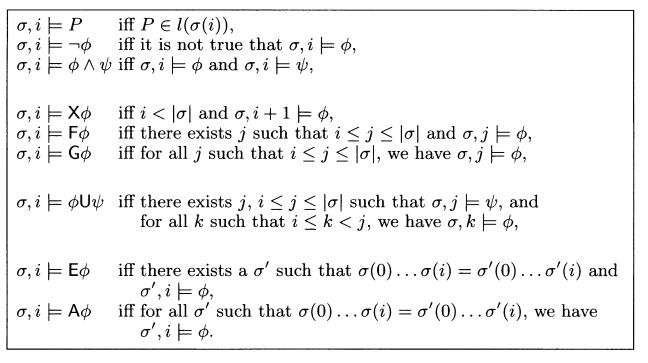
\includegraphics[width=3.5in]{2_3.jpg}
        \caption{Semantics of $\text{CTL}^*$}
    \end{figure}
    
    A derived notion "the automaton $\mathcal{A}$ satisfies $\phi$", denoted $\mathcal{A}\models\phi$ and defined by:
    \begin{equation*}
      \mathcal{A}\models \phi \text{ iff } \sigma,0\models\phi \text{ for every execution } \sigma \text{ of } \mathcal{A}
    \end{equation*}
    
    So far, the fundament of $\text{CTL}^*$ has been introduced. Compared with first-order logic, temporal logic eliminates the parameter $t$ because its formula implies $t$ and breaks the continuous time into discrete one. Therefore, we just need to focus on the instant we want. And another advantage of $\text{CTL}^*$ compared with first-order logic is that it reduces the expressive complexity because the first-order logic needs to write down all the expressions concerned with all the situations. Therefore, $\text{CTL}^*$ is a high level language compiled in machine language. 
    
    In the above section, we have mentioned that in practice, only fragment of $ \text{CTL}^*$ is adopted. Thus PLTL and CTL are proposed to express the executions of a system.
    
    PTLT is a fragment of $\text{CTL}^*$ by dropping $\text{\textbf{A}}$ and $\text{\textbf{E}}$. We have known that $\text{\textbf{A}}$ and $\text{\textbf{E}}$ quantify over the set of executions. After dropping them, thus, PLTL can not distinguish whether the execution out of the state at instant $i$ would split off or not. It means that PLTL can only express "linear time logic".
    
    And CTL remains $\text{\textbf{A}}$ and $\text{\textbf{E}}$ of $\text{CTL}^*$ but it requires that each use of a temporal combinator should be under the immediate scope of path quantifiers. It is the criterion to judge CTL. Therefore, CTL formulas should be in the form such as  $\text{\textbf{E}}\text{\textbf{X}},\text{\textbf{A}}\text{\textbf{X}},\text{\textbf{E}}\_\text{\textbf{U}} \_,\text{\textbf{A}}\_\text{\textbf{U}} \_$ and etc.
    
    Choosing which fragment of $\text{CTL}^*$ is important because each one has its advantages and disadvantages. For PLTL, it is more suitable to state properties of a system while CTL is suited for exhaustive verification of a system. Thus, a compromise depended on several factors is often adopted.
    
    \section{Summary}
    From the illustration above, we have known how to use $\text{CTL}^*$ to express executions of a system depending on which fragment of $\text{CTL}^*$ you use. Compared with first-order logic, $\text{CTL}^*$ is more expressive and simpler for which it weakens the parameter $t$ and can group some first-order into one and thus reduces the complexity of expressions. What we need to pay attention to is just the correct usage of various combinators and quantifiers.
\end{document} 